\section{Background}
\label{background}

\subsection{Machine Learning} \label{background_machinelearning}
\subsubsection{Neural Networks}
\subsubsection{Support Vector Machines}
\subsection{Spaced Repetition} \label{background_spacedrepetition}
\subsubsection*{Supermemo 2 Algorithm (SM2)}
\begin{equation}
I(1) := 1
\end{equation}

\begin{equation}
I(2) := 6
\end{equation}

\begin{equation}
I(n) := I(n-1) \times EF
\end{equation}

\begin{equation}
EF := EF + (0.1 - (5 - q) \times (0.08 + (5 - q) * 0.02))
\end{equation}

\subsection{Similar Projects} \label{background_similarprojects}
\subsubsection*{Memrise}
Memrise is a private company which produces web-based flashcard software.

\subsubsection*{The Mnemosyne Project}
Mnemosyne is open source spaced repetition software collecting anonymised data from its many users in order
to evaluate the effectiveness of the implemented spaced repetition algorithm \cite{peter_bienstman_principles_2012}.
Mnemosyne uses a modified version of the Supermemo algorithm.
The project does not appear to have produced any papers or research publications at this time.

\begin{figure}[h!]
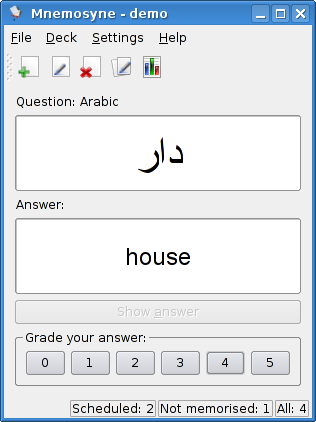
\includegraphics[width=4cm]{img/mnemosyne_screen.png}
\caption{Screenshot of Mnemosyne in use}
\end{figure}

\subsubsection*{Anki}

